\begin{figure*}[t]
    \centering
    \begin{subfigure}[b]{0.325\linewidth}
        \centering
        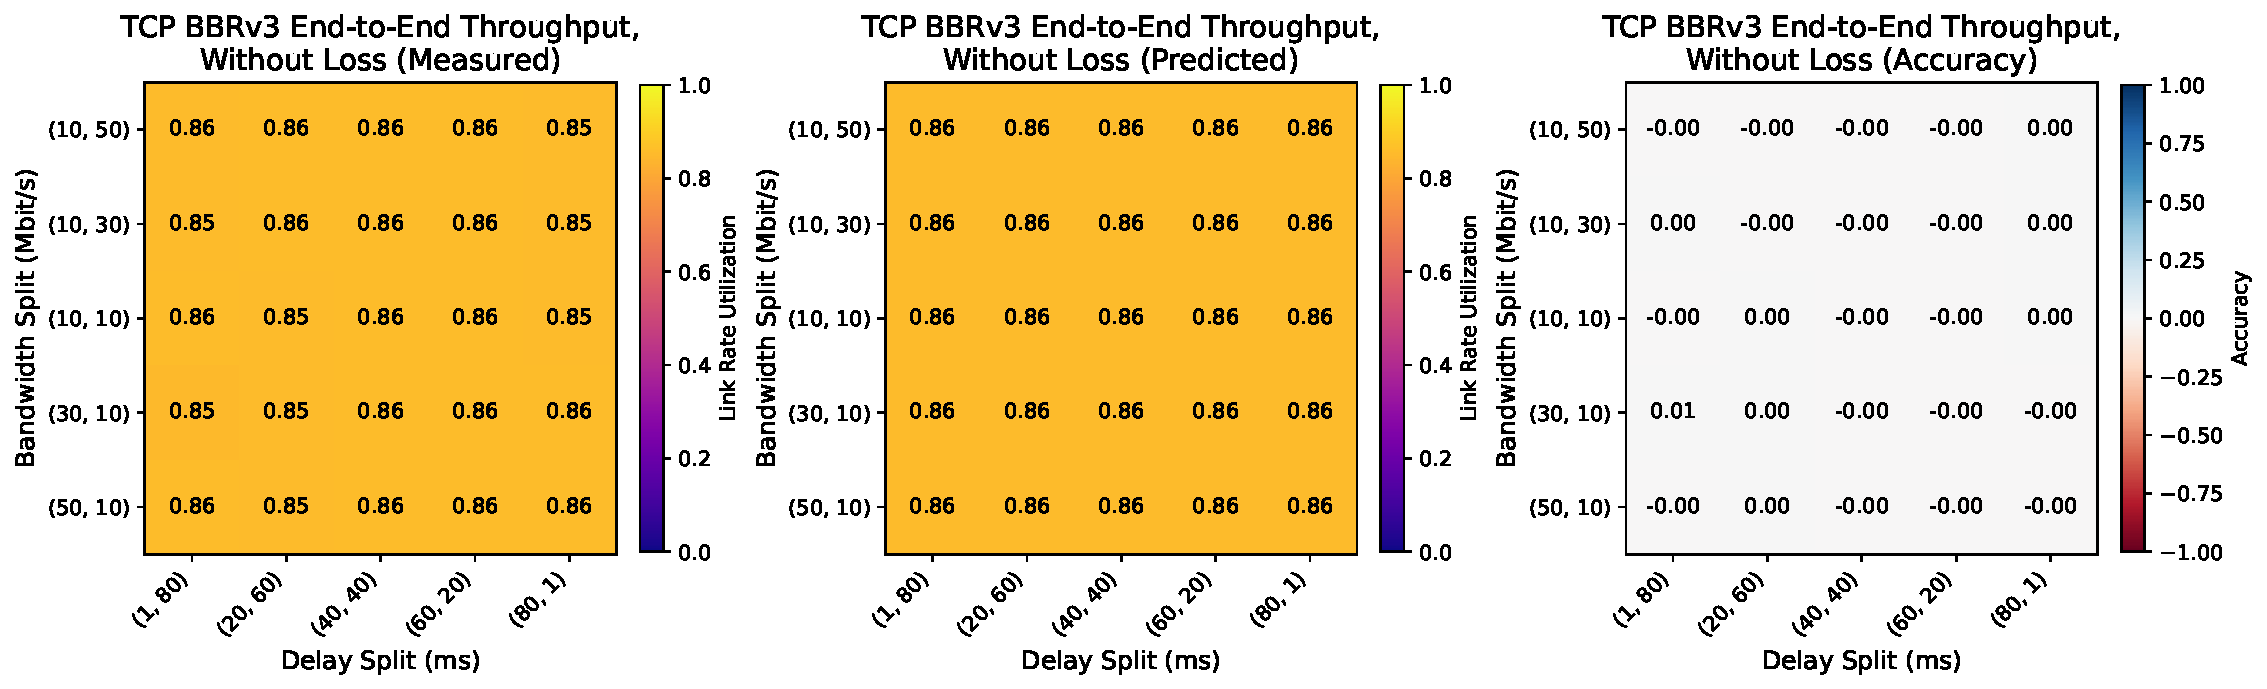
\includegraphics[width=\linewidth,trim={0 0 25.8cm 0},clip]
         {splitting-paper/figures/accuracy/accuracy_e2e_without_loss.pdf}
        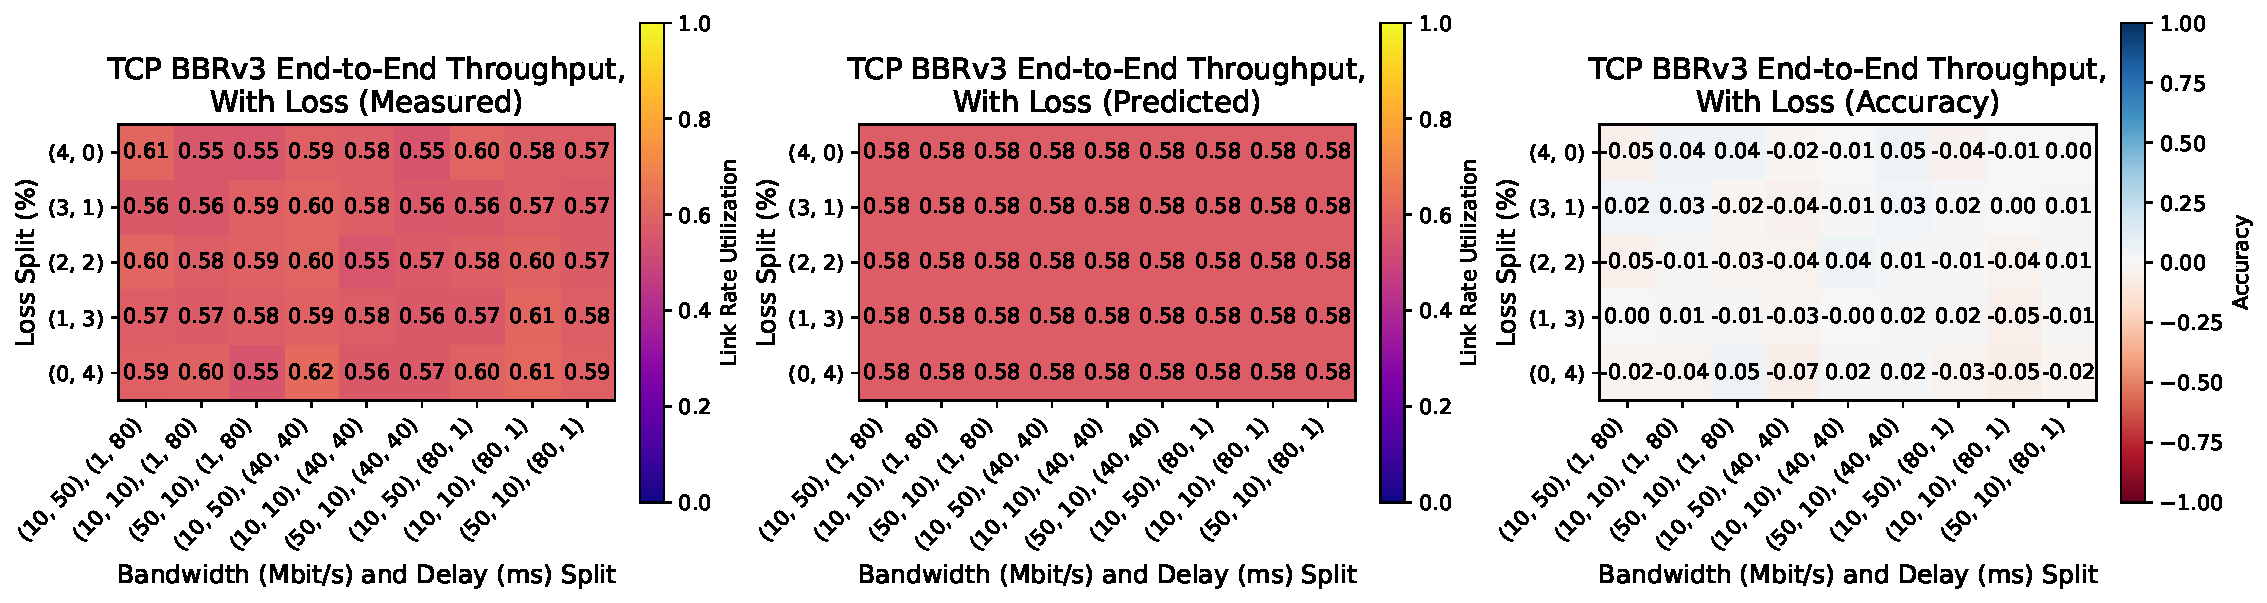
\includegraphics[width=\linewidth,trim={0 0 25.8cm 0},clip]
         {splitting-paper/figures/accuracy/accuracy_e2e_with_loss.pdf}
        \captionsetup{skip=4pt}
        \caption{End-to-end throughput accuracy.}
        \label{fig:accuracy:e2e}
    \end{subfigure}
    \begin{subfigure}[b]{0.645\linewidth}
        \centering
        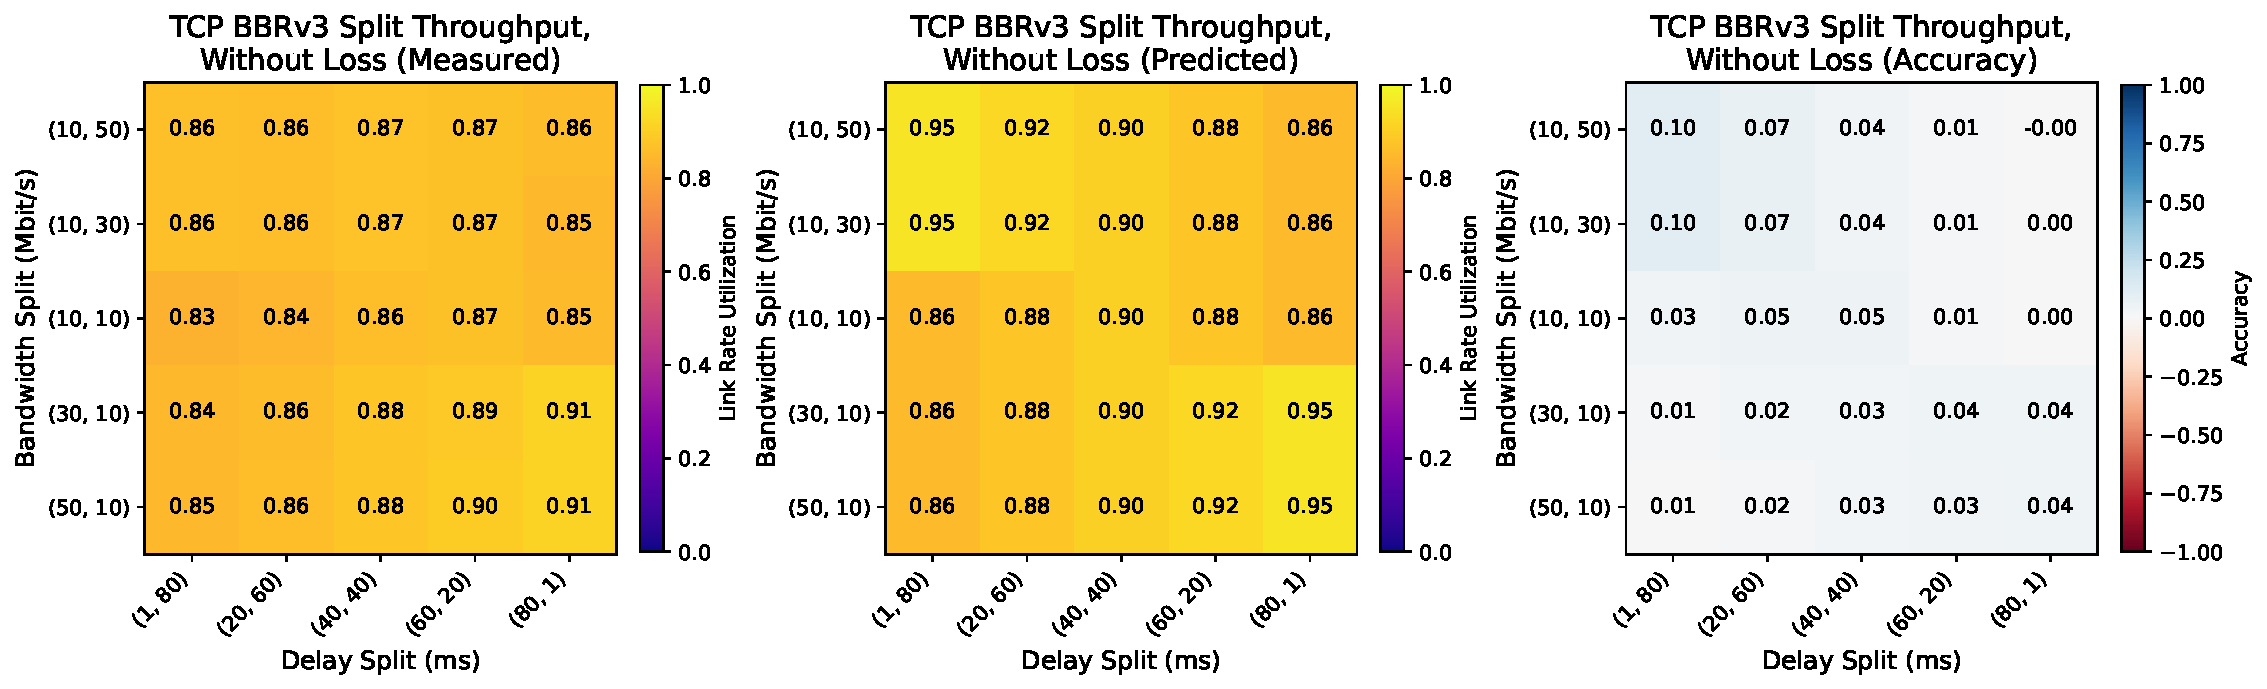
\includegraphics[width=\linewidth,trim={0 0 13.4cm 0},clip]
         {splitting-paper/figures/accuracy/accuracy_split_without_loss.pdf}
        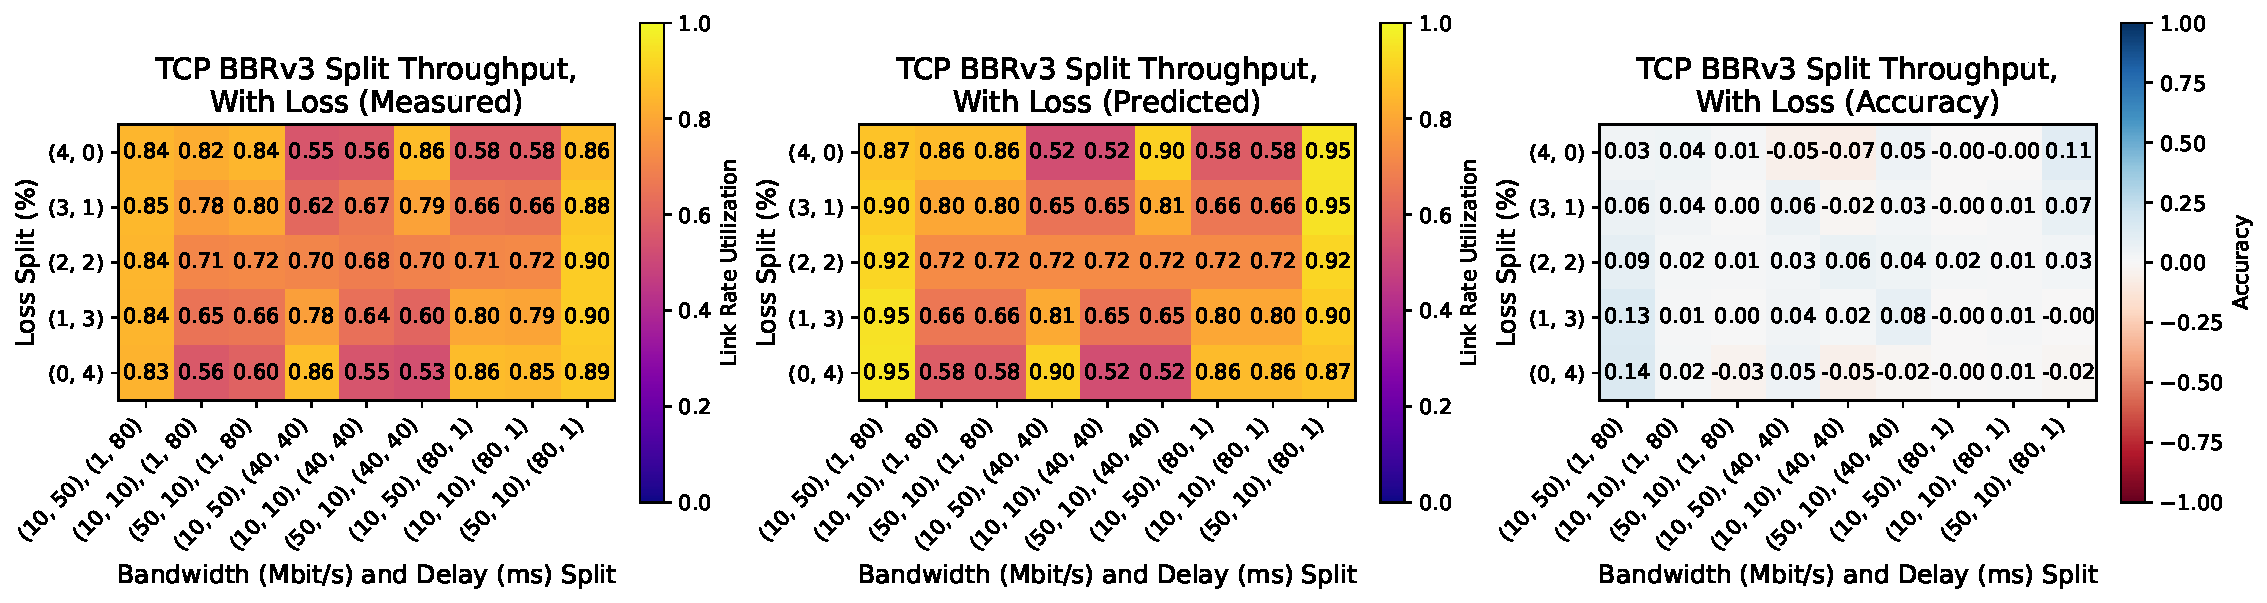
\includegraphics[width=\linewidth,trim={0 0 13.4cm 0},clip]
         {splitting-paper/figures/accuracy/accuracy_split_with_loss.pdf}
        \captionsetup{skip=4pt}
        \caption{Split throughput accuracy.}
        \label{fig:accuracy:split}
    \end{subfigure}

    \caption{Heatmaps of the measured and predicted BBRv3 throughputs for
     various splits of delay, bandwidth, and loss, both without (top) and with
     (bottom) loss.
     The \textit{end-to-end throughput} predictions (not pictured) are the same for all
     cells at 0.86 utilization without loss and 0.58 utilization with loss,
     because they represent the same network path, so end-to-end
     prediction errors are roughly uniform.
     The \textit{split throughput} predictions err slightly on the side of
     overestimation, but they accurately reflect trends in higher or lower throughputs for
     measurements on different splits of the same network path. Median of $n=40$ trials.}
    \label{fig:accuracy}
    \vspace{-0.3cm}
\end{figure*}
